% -------------------------------------
% QUT Mathematics Society
% LaTeX Workshop
% Created by: Tarang Janawalkar (2022)
% -------------------------------------

% -------------------------------------
% Preprocessing directives
% -------------------------------------

% The following 4 lines beginning with `%!` contain preprocessing directives.
% They provide options to the various programs so that the compilation process
% is constant across all platforms.
% These lines are generally placed at the top of the document.

% Biber:
% The following directives should only be enabled when bibliography references
% are modified.
% Otherwise place an additional `%` at the beginning of both lines to disable them,
% or if no bibliography is utilised, remove them completely.
%!BIB program = biber
%!BIB options = --input-directory Debug --output-directory Debug "main.bcf"

% TeX:
% The following directives are used to control the behaviour of the TeX engine.
%!TEX TS-program = xelatex
%!TEX options = -aux-directory=Debug -shell-escape -file-line-error -interaction=nonstopmode -halt-on-error -synctex=1 "%DOC%"

% -------------------------------------
% Preamble
% -------------------------------------

% In the preamble we define the type of document we are writing,
% load additional packages and set various parameters.

% -------------------------------------
%% Document declaration
% -------------------------------------

% This is at the start of every LaTeX document.

% The document class specifies the overall type of document we are writing.
\documentclass[11pt, twoside]{article}
% 'article' is most common.
% 'report' is similar to 'article', but allows for chapters.
% 'book' is for writing large books.
% 'beamer' is for making presentations.

% -------------------------------------
%% Packages
% -------------------------------------

% Packages add extra functionality to default LaTeX by adding
% new macros or changing default behaviours.

%% Page layout
\usepackage[a4paper, margin = 2.5cm]{geometry}  % Controls layout of the page, including margins

%% Mathematical environments and symbols
\usepackage{mathtools}                          % Maths equations and aligns (inherits from amsmath)
\usepackage{amsmath}                            % Misc enhancements to math equations
\usepackage{amssymb}                            % More maths symbols
\usepackage{derivative}                         % Derivative symbols

%% Scientific Notation
\usepackage{siunitx}                            % SI unit typesetting
\usepackage[version=4]{mhchem}                  % Chemical equation typesetting

%% Figures
\usepackage{float}                              % Figure positioning
\usepackage{graphicx}                           % Including images
\usepackage{booktabs}                           % For prettier looking tables
\usepackage{subcaption}                         % For using subfigures
\usepackage{array}                              % Column formatting

%% Source code
\usepackage{minted}                             % Source code layout, formatting and styling
\usepackage{color}                              % Needed for colouring source code syntax

%% References
\usepackage[style=apa]{biblatex}                % Controls bibliography and citations
\usepackage[hidelinks]{hyperref}                % Support for links. Autolinks citations, references, and TOC

%% Lists
\usepackage{enumitem}                           % List environments

%% Unicode support
\usepackage[warnings-off={mathtools-colon, mathtools-overbracket}]{unicode-math}

%% Menukey and directory path formatting
\usepackage{menukeys}

%% Create boxed environments
\usepackage{tcolorbox}

% -------------------------------------
%% Global settings
% -------------------------------------

\setminted[tex]{
	frame=lines,                 % Frame lines
	linenos,                     % Line numbers
    breaklines                   % Break lines
}

% Custom box for displaying example outputs in this document
\newtcolorbox{outputbox}[1][]{
    colback=white,
    title=Output,
    #1
}

%% Extra operator example
\DeclareMathOperator{\proj}{proj}

%% Font used by QUT (remove to use original TeX font)
\setmainfont{TeX Gyre Pagella}
\setmathfont{TeX Gyre Pagella Math}

% Hide \vbox underfull warnings for the workshop
\raggedbottom

% -------------------------------------
%% Miscellaneous settings
% -------------------------------------

% Add the references to the bibliography
\addbibresource{sample.bib}

% -------------------------------------
% Title page setup
% -------------------------------------

\title{\LaTeX{} Workshop}
\author{QUT Maths Society}

% Date setup
                    % if nothing is provided, LaTeX uses current date
% \date{6 April 2022} % Specific date
% \date{}             % No date

% -------------------------------------
% End of Preamble
% -------------------------------------

% -------------------------------------
% Document content
% -------------------------------------

% Start of document content
\begin{document}

% -------------------------------------
%% Title page and ToC
% -------------------------------------

% Places the title, author, and date.
\maketitle

% Page number style for the table of contents
\pagenumbering{roman}

% Places the table of contents which is generated automatically
% from the sections
\tableofcontents

% List of images/tables are also generated automatically
\listoffigures
\listoftables

% Inserts a new page
\newpage
\pagenumbering{arabic}

% -------------------------------------
%% Document main content
% -------------------------------------

\section{Introduction}
``\LaTeX{} is a high-quality typesetting system; it includes features
designed for the production of technical and scientific documentation.
\LaTeX{} is the de facto standard for the communication and publication
of scientific documents. \LaTeX{} is available as free software'' \parencite{latex_project_latex}.

One of the key differences between \LaTeX{} and more common word
processors such as MS Word, LibreOffice etc., is the separation of
content and presentation. In \LaTeX{}, the author describes the general
structure of the document (i.e., section headings, paragraphs,
equations, and figures), and the layout and typesetting are handled by
\LaTeX{} (or rather the underlying \TeX{} backend).

There are several advantages to this:
\begin{itemize}
    \item The author can focus on the actual content without worrying
          about layout and presentation
    \item The presentation can be modified without introducing major
          changes to the document
    \item \LaTeX{}'s standard format allows authors to easily conform to
          styles provided by external publishers
\end{itemize}
\LaTeX{} is written in plaintext and processed by an external program to
generate output files (usually PDFs).
\subsection{Pronunciation and Spelling}
\LaTeX{} is pronounced \emph{lah-tech} or \emph{lay-tech}, but \TeX{} is
never pronounced \emph{tecks}. It is typeset using the
\mintinline{tex}{\LaTeX{}} macro or with the capitalisation ``LaTeX''.
\subsection{Language Structures}
There are two major language structures that we encounter when using
\LaTeX{}; \textit{macros} and \textit{environments}.
\subsubsection{Macros}
Macros (or commands) tell \LaTeX{} how to do things. They use the
following syntax
\begin{minted}{tex}
\commandname
% or
\commandname[optional args]{required args}
\end{minted}
Macros provide functionality for layouts, symbols, styles, etc. As
shown below, common font styles can be invoked using macros.
\begin{description}
    \item[Bold face] \mintinline{tex}|\textbf{Text}| --- \textbf{Text}
    \item[Italics] \mintinline{tex}|\textit{Text}| --- \textit{Text}
    \item[Emphasis] \mintinline{tex}|\emph{Text}| --- \emph{Text}
          (either upright or italics depending on surrounding text)
    \item[Underline] \mintinline{tex}|\underline{Text}| ---
          \underline{Text}
\end{description}
We can also define custom macros that combine other macros or simplify repetitive instructions.
\begin{minted}{tex}
\newcommand{\commandname}[number_of_arguments]{command_body}
\end{minted}
Arguments can be referenced inside the command body with the
\mintinline{tex}{#argument_number} syntax. For example
\begin{minted}{tex}
\newcommand{\boldanditalics}[1]{\textbf{\textit{#1}}}
\boldanditalics{Bold and italics text}
\end{minted}
\newcommand{\boldanditalics}[1]{\textbf{\textit{#1}}}
\begin{outputbox}
    \boldanditalics{Bold and italics text}
\end{outputbox}
\subsubsection{Environments}
Environments are used to format large blocks of text which often
contain many lines or multiple macros. Environments use opening
\mintinline{tex}{\begin} and closing \mintinline{tex}{\end} tags so % chktex 14
that everything inside those tags will be formatted in a special manner
depending on the type of the environment.
\begin{minted}{tex}
\begin{environment_name}[optional_arguments]{required_arguments}
    ...
\end{environment_name}
\end{minted}
Common environments include \mintinline{tex}{figure},
\mintinline{tex}{equation}, \mintinline{tex}{itemize} (these will be
discussed later), etc.\ \newpage
\section{Basic Structure}
\subsection{Sections}
Sections are used to divide the document into parts. A new section is
started with the \mintinline{tex}{\section} macro. Section titles are
formatted to be bold and larger than regular text. The number preceding
the title is automatically determined.

The table of contents (\mintinline{tex}{\tableofcontents}) is also
generated from these section macros, so that page numbers and section
numbers are set automatically.
\subsection{Subsections}
We can split sections into smaller subsections \mintinline{tex}|\subsection{Subsections}|,
\subsubsection{Subsubsections}
and also subsubsections \mintinline{tex}|\subsubsection{Subsubsections}|.
\subsection*{Unnumbered sections}
\addcontentsline{toc}{subsection}{Unumbered sections}
We can remove section numbering by using the starred version of the
section macro i.e., \linebreak \mintinline{tex}|\subsection*{Unnumbered sections}|.
As this also removes the section from the table of contents, we can
manually add it using
\begin{minted}{tex}
\addcontentsline{toc}{subsection}{Unumbered sections}
\end{minted}
remembering to place this immediately after the section macro so that
the reference is set to the correct location.
\subsection{Lists}
Unordered (bullet) lists are produced by the \mintinline{tex}{itemize}
environment, where each list entry starts by using the
\mintinline{tex}{\item} macro, which also generates the bullet symbol.
\begin{minted}{tex}
\begin{itemize}
    \item List entries ...
    \item We can ...
          \begin{itemize}
              \item We can ...
                    \begin{itemize}
                        \item The marker ...
                              \begin{itemize}
                                  \item List markers, ...
                              \end{itemize}
                    \end{itemize}
          \end{itemize}
\end{itemize}
\end{minted}
\begin{outputbox}
    \begin{itemize}
        \item List entries start with the \mintinline{tex}{\item} macro
              and are indicated by the black dot
        \item We can create multiple entries
              \begin{itemize}
                  \item We can nest lists by creating another
                        \mintinline{tex}{itemize} environment
                        \begin{itemize}
                            \item The marker changes in each nested
                                  list to reflect the depth
                                  \begin{itemize}
                                      \item List markers, spacing, and
                                            other behaviour can be
                                            customised with the
                                            \mintinline{tex}{enumitem}
                                            package
                                  \end{itemize}
                        \end{itemize}
              \end{itemize}
    \end{itemize}
\end{outputbox}
Numbered (ordered) lists use the same syntax as unordered lists but use
the \mintinline{tex}{enumerate} environment.
\begin{minted}{tex}
\begin{enumerate}
    \item List entries ...
    \item Nested lists ...
          \begin{enumerate}
              \item But use ...
                    \begin{enumerate}
                        \item Such as ...
                    \end{enumerate}
          \end{enumerate}
\end{enumerate}
\end{minted}
\begin{outputbox}
    \begin{enumerate}
        \item List entries are numbered automatically
        \item Nested lists are also numbered
              \begin{enumerate}
                  \item But use a different number format
                        \begin{enumerate}
                            \item Such as lowercase letters and roman
                                  numerals
                        \end{enumerate}
              \end{enumerate}
    \end{enumerate}
\end{outputbox}
We can change the top-level number format by specifying a value to the
\mintinline{tex}{label} parameter.
\begin{minted}{tex}
\begin{enumerate}[label=label_specifier]
    \item ...
\end{enumerate}
\end{minted}
The following label specifiers can be used to override the default
numbering format:
\begin{enumerate}[label=\arabic*.]
    \item --- \mintinline{tex}{[label=\arabic*.]} (Default)
\end{enumerate}
\begin{enumerate}[label=<\Roman*>]
    \item --- \mintinline{tex}{[label=<\Roman*>]}
\end{enumerate}
\begin{enumerate}[label=\roman*]
    \item --- \mintinline{tex}{[label=\roman*]}
\end{enumerate}
\begin{enumerate}[label=(\alph*)]
    \item --- \mintinline{tex}{[label=(\alph*)]}
\end{enumerate}
\begin{enumerate}[label=Part \Alph*:]
    \item --- \mintinline{tex}{[label=Part \Alph*:]}
\end{enumerate}
\newpage
\section{Mathematics}
One of \LaTeX{}'s strengths is how it formats mathematical expressions.
There are two ways to format mathematical expressions; inline using
\mintinline{tex}{\( \)} and display style using \mintinline{tex}{\[ \]}.

Mathematical expressions can be contained ``inline'' (within) text and
require less space:
\begin{minted}{tex}
Let \(\mathbb{N}\) denote the set of all natural numbers.
\end{minted}
\begin{outputbox}
    Let \(\mathbb{N}\) denote the set of all natural numbers.
\end{outputbox}
Mathematical expressions typeset outside paragraph text appear as standalone, display style math:
\begin{minted}{tex}
\[
    \lim_{\Delta{t} \to \infty} \frac{f\left( t + \Delta{t} \right) - f\left( t \right)}{\Delta{t}}
\]
\end{minted}
\begin{outputbox}
    \[
        \lim_{\Delta{t} \to \infty} \frac{f\left( t + \Delta{t} \right) - f\left( t \right)}{\Delta{t}}
    \]
\end{outputbox}
Note that we commonly use \mintinline{tex}{\equation} environments for automatic vertical spacing and equation numbering
(as with section headings).
\begin{minted}{tex}
\begin{equation}
    a^2 + b^2 = c^2
\end{equation}
\end{minted}
\begin{outputbox}
    \begin{equation}
        a^2 + b^2 = c^2
    \end{equation}
\end{outputbox}
We can use the starred version of this environment to remove the equation label.
\begin{minted}{tex}
\begin{equation*}
    a^2 + b^2 = c^2
\end{equation*}
\end{minted}
\begin{outputbox}
    \begin{equation*}
        a^2 + b^2 = c^2
    \end{equation*}
\end{outputbox}
\subsection{Paired Delimiters}
\begin{table}[H]
    \centering
    \begingroup
    \renewcommand{\arraystretch}{1.2}
    \begin{tabular}{c c c c}
        \toprule
        \textbf{Name}  & \textbf{\LaTeX{} Command}                      & \textbf{Inline}                  & \textbf{Display Style}                         \\
        \midrule
        Parentheses    & \mintinline{tex}{\left( a \right)}             & \(\left( a \right)\)             & \(\displaystyle \left( a \right)\)             \\ % chktex 37
        Brackets       & \mintinline{tex}{\left[ a \right]}             & \(\left[ a \right]\)             & \(\displaystyle \left[ a \right]\)             \\
        Braces         & \mintinline{tex}|\left\{ a \right\}|           & \(\left\{ a \right\}\)           & \(\displaystyle \left\{ a \right\}\)           \\
        Angle brackets & \mintinline{tex}{\left\langle a \right\rangle} & \(\left\langle a \right\rangle\) & \(\displaystyle \left\langle a \right\rangle\) \\
        Pipes          & \mintinline{tex}{\left\lvert a \right\lvert}   & \(\left\lvert a \right\lvert\)   & \(\displaystyle \left\lvert a \right\lvert\)   \\
        Double Pipes   & \mintinline{tex}{\left\lVert a \right\lVert}   & \(\left\lVert a \right\lVert\)   & \(\displaystyle \left\lVert a \right\lVert\)   \\
        Ceiling        & \mintinline{tex}{\left\lceil a \right\rceil}   & \(\left\lceil a \right\rceil\)   & \(\displaystyle \left\lceil a \right\rceil\)   \\
        Floor          & \mintinline{tex}{\left\lfloor a \right\rfloor} & \(\left\lfloor a \right\rfloor\) & \(\displaystyle \left\lfloor a \right\rfloor\) \\
        \bottomrule
    \end{tabular}
    \endgroup
    \caption{Paired Delimiters in \LaTeX{}.} % \label{}
\end{table}
Note that we can declare custom paired delimiters for the final five examples using the following syntax:
\begin{minted}{tex}
\DeclarePairedDelimiter{\paired_delimiter_name}{left_delimiter}{right_delimiter}
\end{minted}
Here are a few suggestions
\begin{minted}{tex}
\DeclarePairedDelimiter{\ceil}{\lceil}{\rceil}
\DeclarePairedDelimiter{\floor}{\lfloor}{\rfloor}
\DeclarePairedDelimiter{\abracket}{\langle}{\rangle}
\DeclarePairedDelimiter{\abs}{\lvert}{\rvert}
\DeclarePairedDelimiter{\norm}{\lVert}{\rVert}
\end{minted}
\DeclarePairedDelimiter{\ceil}{\lceil}{\rceil}
\DeclarePairedDelimiter{\floor}{\lfloor}{\rfloor}
\DeclarePairedDelimiter{\abracket}{\langle}{\rangle}
\DeclarePairedDelimiter{\abs}{\lvert}{\rvert}
\DeclarePairedDelimiter{\norm}{\lVert}{\rVert}
\subsection{Arithmetic Operators}
\begin{table}[H]
    \centering
    \begingroup
    \renewcommand{\arraystretch}{1.2}
    \begin{tabular}{c c c c}
        \toprule
        \textbf{Name}  & \textbf{\LaTeX{} Command}                           & \textbf{Inline}                       & \textbf{Display Style}                              \\
        \midrule
        Addition       & \mintinline{tex}{a + b}                             & \(a + b\)                             & \(\displaystyle a + b\)                             \\
        Subtraction    & \mintinline{tex}{a - b}                             & \(a - b\)                             & \(\displaystyle a - b\)                             \\ % chktex 8
        Multiplication & \mintinline{tex}{a \cdot \left( b \times c \right)} & \(a \cdot \left( b \times c \right)\) & \(\displaystyle a \cdot \left( b \times c \right)\) \\ % chktex 37
        Inequalities   & \mintinline{tex}{a \ll b < c \leq d}                & \(a \ll b < c \leq d\)                & \(\displaystyle a \ll b < c \leq d\)                \\
        Fractions      & \mintinline{tex}|\frac{a}{b}|                       & \(\frac{a}{b}\)                       & \(\displaystyle \frac{a}{b}\)                       \\
        Superscripts   & \mintinline{tex}{a^2}                               & \(a^2\)                               & \(\displaystyle a^2\)                               \\
        Subscripts     & \mintinline{tex}{a_i}                               & \(a_i\)                               & \(\displaystyle a_i\)                               \\
        Square root    & \mintinline{tex}|\sqrt{a}|                          & \(\sqrt{a}\)                          & \(\displaystyle \sqrt{a}\)                          \\
        \bottomrule
    \end{tabular}
    \endgroup
    \caption{Arithmetic operators in \LaTeX{}.} % \label{}
\end{table}
\subsection{Common Large Operators}
\begin{table}[H]
    \centering
    \begingroup
    \renewcommand{\arraystretch}{2.2}
    \begin{tabular}{c c c c}
        \toprule
        \textbf{Name} & \textbf{\LaTeX{} Command}                           & \textbf{Inline}                       & \textbf{Display Style}                              \\
        \midrule
        Summations    & \mintinline{tex}|\sum_{n = 1}^\infty \frac{1}{n^s}| & \(\sum_{n = 1}^\infty \frac{1}{n^s}\) & \(\displaystyle \sum_{n = 1}^\infty \frac{1}{n^s}\) \\
        Limits        & \mintinline{tex}|\lim_{x \to \infty} \frac{1}{x}|   & \(\lim_{x \to \infty} \frac{1}{x}\)   & \(\displaystyle \lim_{x \to \infty} \frac{1}{x}\)   \\
        Derivatives   & \mintinline{tex}|\odv[order=2]{f}{x} \pdv*{f}{t}|   & \(\odv[order=2]{f}{x} \pdv*{f}{t}\)   & \(\displaystyle \odv[order=2]{f}{x} \pdv*{f}{t}\)   \\
        Integrals     & \mintinline{tex}|\int_0^\infty e^{-x^2} \odif{x}|   & \(\int_0^\infty e^{-x^2} \odif{x}\)   & \(\displaystyle \int_0^\infty e^{-x^2} \odif{x}\)   \\
        Union         & \mintinline{tex}|\bigcup_{i = 1}^n S_i|             & \(\bigcup_{i=1}^n S_i\)               & \(\displaystyle \bigcup_{i=1}^n S_i\)               \\
        \bottomrule
    \end{tabular}
    \endgroup
    \caption{Common large operators in \LaTeX{}.} % \label{}
\end{table}
\subsection{Common Mathematical Functions}
\begin{table}[H]
    \centering
    \begingroup
    \renewcommand{\arraystretch}{1.2}
    \begin{tabular}{c c c c}
        \toprule
        \textbf{Name}     & \textbf{\LaTeX{} Command}                   & \textbf{Inline}               & \textbf{Display Style}                      \\
        \midrule
        Sine              & \mintinline{tex}|\sin{\left( x \right)}|    & \(\sin{\left( x \right)}\)    & \(\displaystyle \sin{\left( x \right)}\)    \\ % chktex 37
        Inverse Sine      & \mintinline{tex}|\arcsin{\left( x \right)}| & \(\arcsin{\left( x \right)}\) & \(\displaystyle \arcsin{\left( x \right)}\) \\ % chktex 37
        Logarithm         & \mintinline{tex}|\log{\left( x \right)}|    & \(\log{\left( x \right)}\)    & \(\displaystyle \log{\left( x \right)}\)    \\ % chktex 37
        Natural Logarithm & \mintinline{tex}|\ln{\left( x \right)}|     & \(\ln{\left( x \right)}\)     & \(\displaystyle \ln{\left( x \right)}\)     \\ % chktex 37
        Exponential       & \mintinline{tex}|\exp{\left( x \right)}|    & \(\exp{\left( x \right)}\)    & \(\displaystyle \exp{\left( x \right)}\)    \\ % chktex 37
        \bottomrule
    \end{tabular}
    \endgroup
    \caption{Common large operators in \LaTeX{}.} % \label{}
\end{table}
\subsection{Multi-line Equations}
As \mintinline{tex}{equation} only allows single line equations, we can
use other environments to group multiple equations into one
environment.
\subsubsection{Gather}
The \mintinline{tex}{gather} environment allows us to display a set of
consecutive equations with multiple lines. New lines are separated
using \mintinline{tex}{\\}.
\begin{minted}{tex}
\begin{gather}
    \sum_{i = 0}^n f\left( i \right) = f\left( 0 \right) + f\left( 1 \right) + \cdots + f\left( n \right) \\
    \prod_{i = 0}^n f\left( i \right) = f\left( 0 \right) \times f\left( 1 \right) \times \cdots \times f\left( n \right)
\end{gather}
\end{minted}
\begin{outputbox}
    \begin{gather}
        \sum_{i = 0}^n f\left( i \right) = f\left( 0 \right) + f\left( 1 \right) + \cdots + f\left( n \right) \\
        \prod_{i = 0}^n f\left( i \right) = f\left( 0 \right) \times f\left( 1 \right) \times \cdots \times f\left( n \right)
    \end{gather}
\end{outputbox}
\newpage
\subsubsection{Align}
The \mintinline{tex}{align} environment allows us to display
consecutive equations that are also aligned. The alignment is
determined by the placement of the \mintinline{tex}{&} character. This
alignment character breaks the equation into ``columns'' that are
either right or left aligned, following the pattern:
\mintinline{tex}{rlrlrl}\dots.
\begin{minted}{tex}
\begin{align}
%   R &  L  & R & L & R & L &  R  & L
    R & = L & R & = & = & L & R = & L
\end{align}
\end{minted}
\begin{outputbox}
    \begin{align}
        R & = L & R & = & = & L & R = & L
    \end{align}
\end{outputbox}
This can be illustrated using a table where the ampersands (\mintinline{tex}{&}) are horizontally aligned with the pipes (\mintinline{tex}{|}).
\begin{table}[H]
    \centering
    \begin{tabular}
        {wc{4.2em}@{\makebox[\widthof{\&}][c]{{\color{blue}|}}}wc{4.2em}@{\makebox[\widthof{\&}][c]{{\color{blue}|}}}wc{4.2em}@{\makebox[\widthof{\&}][c]{{\color{blue}|}}}wc{4.2em}@{\makebox[\widthof{\&}][c]{{\color{blue}|}}}wc{4.2em}@{\makebox[\widthof{\&}][c]{{\color{blue}|}}}wc{4.2em}@{\makebox[\widthof{\&}][c]{{\color{blue}|}}}wc{4.2em}@{\makebox[\widthof{\&}][c]{{\color{blue}|}}}wc{4.2em}} % chktex 44
        Right & Left & Right & Left & Right & Left & Right & Left \\
        \midrule
    \end{tabular}
    \begin{tabular}
        {wr{4.2em}@{{\color{blue}\&}}wl{4.2em}@{{\color{blue}\&}}wr{4.2em}@{{\color{blue}\&}}wl{4.2em}@{{\color{blue}\&}}wr{4.2em}@{{\color{blue}\&}}wl{4.2em}@{{\color{blue}\&}}wr{4.2em}@{{\color{blue}\&}}wl{4.2em}}
        \(R\) & \(= L\) & \(R\) & \(=\) & \(=\) & \(L\) & \(R =\) & \(L\) \\
    \end{tabular}
    % \caption{} % \label{}
\end{table}
With this in mind, we can create aligned equations as shown below.
\begin{align}
    ax^2 + bx + c                                                    & = 0                                  \\
    a\left( x^2 + \frac{b}{a}x + \frac{c}{a} \right)                 & = 0                                  \\
    x^2 + \frac{b}{a}x + \left( \frac{b}{2a} \right)^2 + \frac{c}{a} & = \left( \frac{b}{2a} \right)^2      \\
    \left( x + \frac{b}{2a} \right)^2                                & = \frac{b^2}{4a^2} - \frac{c}{a}     \\
    x + \frac{b}{2a}                                                 & = \frac{\pm \sqrt{b^2 - 4ac}}{2a}    \\
    x                                                                & = \frac{-b \pm \sqrt{b^2 - 4ac}}{2a}
\end{align}
\begin{align*}
    \symbf{v}_1 & = \symbf{w}_1                                                                                                   & \symbf{q}_1 & = \frac{\symbf{v}_1}{\norm{\symbf{v}_1}} \\
    \symbf{v}_2 & = \symbf{w}_2 - \proj_{\symbf{q}_1} \left( \symbf{w}_2 \right)                                                  & \symbf{q}_2 & = \frac{\symbf{v}_2}{\norm{\symbf{v}_2}} \\
    \symbf{v}_3 & = \symbf{w}_3 - \proj_{\symbf{q}_1} \left( \symbf{w}_3 \right) - \proj_{\symbf{q}_2} \left( \symbf{w}_3 \right) & \symbf{q}_3 & = \frac{\symbf{v}_3}{\norm{\symbf{v}_3}} \\
                & \vdots                                                                                                          &             & \vdots                                   \\
    \symbf{v}_i & = \symbf{w}_i - \sum_{j = 1}^{i - 1} \proj_{\symbf{q}_j} \left( \symbf{w}_i \right)                             & \symbf{q}_i & = \frac{\symbf{v}_i}{\norm{\symbf{v}_i}}
\end{align*}
\pagebreak
\subsection{Text Mode}
If we want to write normal text in math mode, we need to use the
\mintinline{tex}{\text} macro.
\begin{minted}{tex}
\begin{align*}
    \text{Text in text mode} \\
    Text in math mode
\end{align*}
\end{minted}
\begin{outputbox}
    \begin{align*}
        \text{Text in text mode} \\
        Text in math mode
    \end{align*}
\end{outputbox}
Notice that spaces are ignored in math mode.
\subsection{Additional Environments \& Symbols}
The \mintinline{tex}{amsmath} package also allows us to use many matrix
environments using:
\begin{itemize}
    \item \mintinline{tex}{matrix} for a matrix without any enclosing symbols
    \item \mintinline{tex}{pmatrix} for parentheses
    \item \mintinline{tex}{bmatrix} for brackets
    \item \mintinline{tex}{Bmatrix} for braces
    \item \mintinline{tex}{vmatrix} for pipes
    \item \mintinline{tex}{Vmatrix} for double pipes
\end{itemize}
\begin{outputbox}

    \begin{equation*}
        \begin{matrix}
            a & b \\
            c & d
        \end{matrix}
        \quad
        \begin{pmatrix}
            a & b \\
            c & d
        \end{pmatrix}
        \quad
        \begin{bmatrix}
            a & b \\
            c & d
        \end{bmatrix}
        \quad
        \begin{Bmatrix}
            a & b \\
            c & d
        \end{Bmatrix}
        \quad
        \begin{vmatrix}
            a & b \\
            c & d
        \end{vmatrix}
        \quad
        \begin{Vmatrix}
            a & b \\
            c & d
        \end{Vmatrix}
    \end{equation*}
\end{outputbox}
\LaTeX{} provides lots of symbols that can be installed from the \href{https://ctan.org}{Comprehensive TeX Archive Network} that are used in math mode, including the greek alphabet (shown below). A short (but extensive) list can be found at \href{https://www.rpi.edu/dept/arc/training/latex/LaTeX_symbols.pdf}{The Great, Big List of \LaTeX{} Symbols}.
\begin{equation*}
    \alpha \beta \gamma \delta \epsilon \varepsilon \zeta \eta \theta \vartheta \iota \kappa \lambda \mu \nu \xi \pi \varpi \rho \varrho \sigma \varsigma \tau \upsilon \phi \varphi \chi \psi \omega
\end{equation*}
\begin{equation*}
    \Gamma \Delta \Theta \Lambda \Xi \Pi \Sigma \Upsilon \Phi \Psi \Omega
\end{equation*}
Bringing all of these together can give pretty equations like:
\begin{equation*}
    \Gamma\left( z \right) = \int_0^\infty t^{z - 1} e^{-t} \odif{t} = \frac{e^{-\gamma z}}{z} \prod_{k = 1}^\infty \left( 1 + \frac{z}{k} \right)^{-1} e^{\frac{z}{k}}
\end{equation*}
\begin{equation*}
    \symbf{G}_{\mu \nu} + \symbf{\Lambda} \symbf{g}_{\mu \nu} = \kappa \symbf{T}_{\mu \nu}
\end{equation*}
\begin{equation*}
    \ce{Hg^2+ ->[I-] HgI2 ->[I-] [Hg^{II}I4]^2-}
\end{equation*}
\begin{equation}
    \label{eq:schrodingers_equation}
    i \hbar \pdv*{\Psi\left( x,\: t \right)}{t} = -\frac{\hbar^2}{2m} \pdv[order=2]{}{x} \Psi\left( x,\: t \right) + V\left( x,\: t \right) \Psi\left( x,\: t \right)
\end{equation}
\newpage
\section{Figures, Tables, and Code}
\subsection{Figures and Tables}\label{sec:figures_and_tables}
\LaTeX{} allows us to use figures and tables which can be added raw or by using floats.
We generally use floats to allow \LaTeX{} to algorithmically place figures on a page, and
move to the next page if it encounters a vertical overflow.

The float environment for figures is \mintinline{tex}{figure} and
\mintinline{tex}{table} for tables. Floats are containers for objects
that cannot be displayed over multiple pages. They should always have a
descriptive caption (\mintinline{tex}{\caption}) so that the reader
does not have to rely on the contents, and also so that we can
reference them using hyperlinks.
\begin{minted}{tex}
\begin{figure}[H]
    \centering
    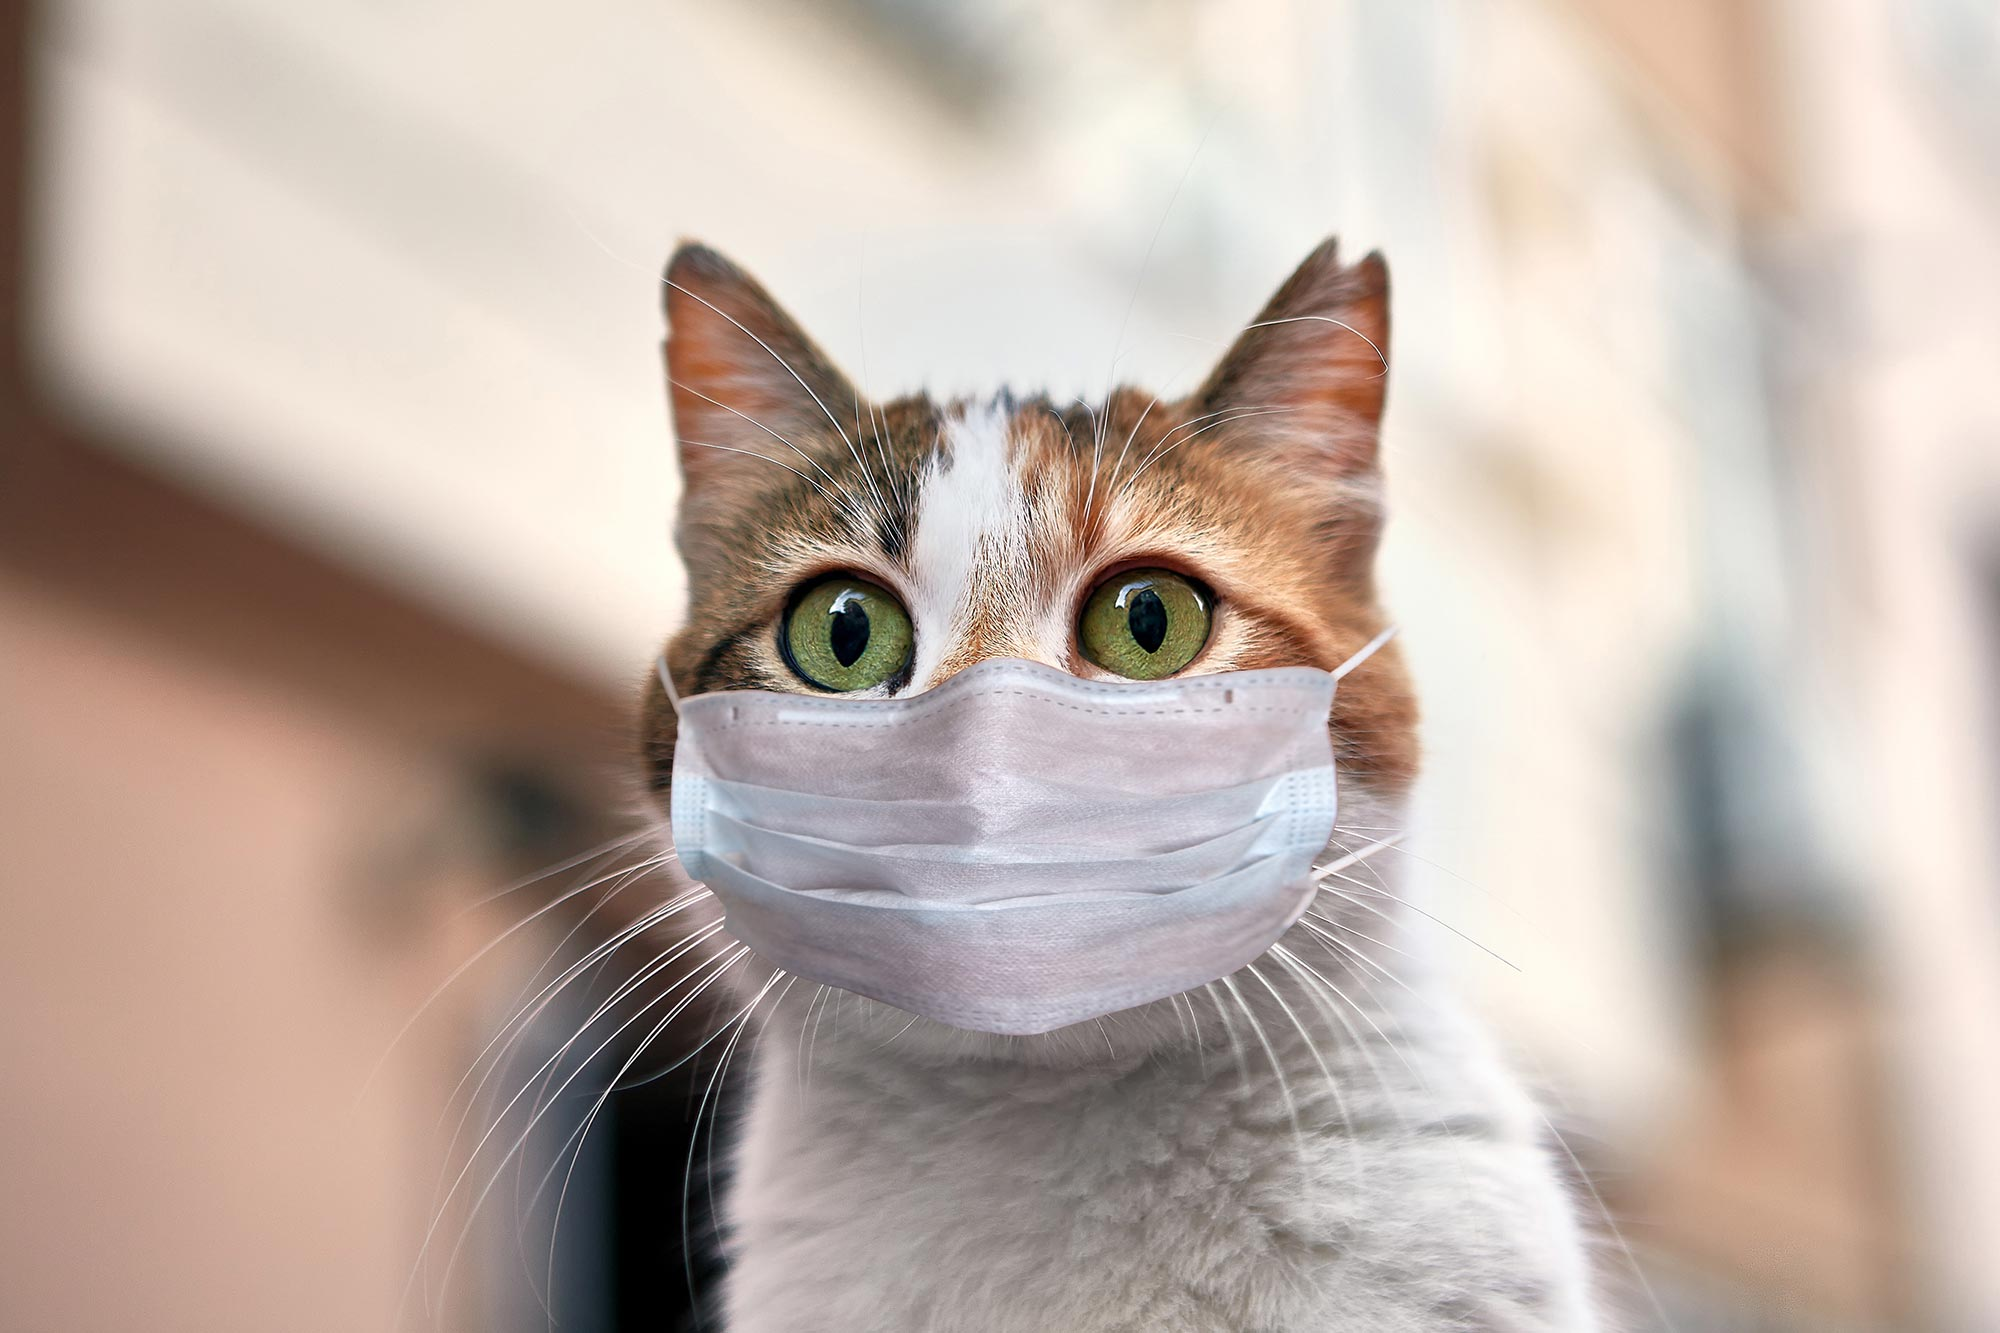
\includegraphics[width=0.5\linewidth]{images/cat.jpg}
    \caption{This is a description of the figure.}\label{fig:cat}
\end{figure}
\end{minted}
\begin{outputbox}
    \begin{figure}[H]
        \centering
        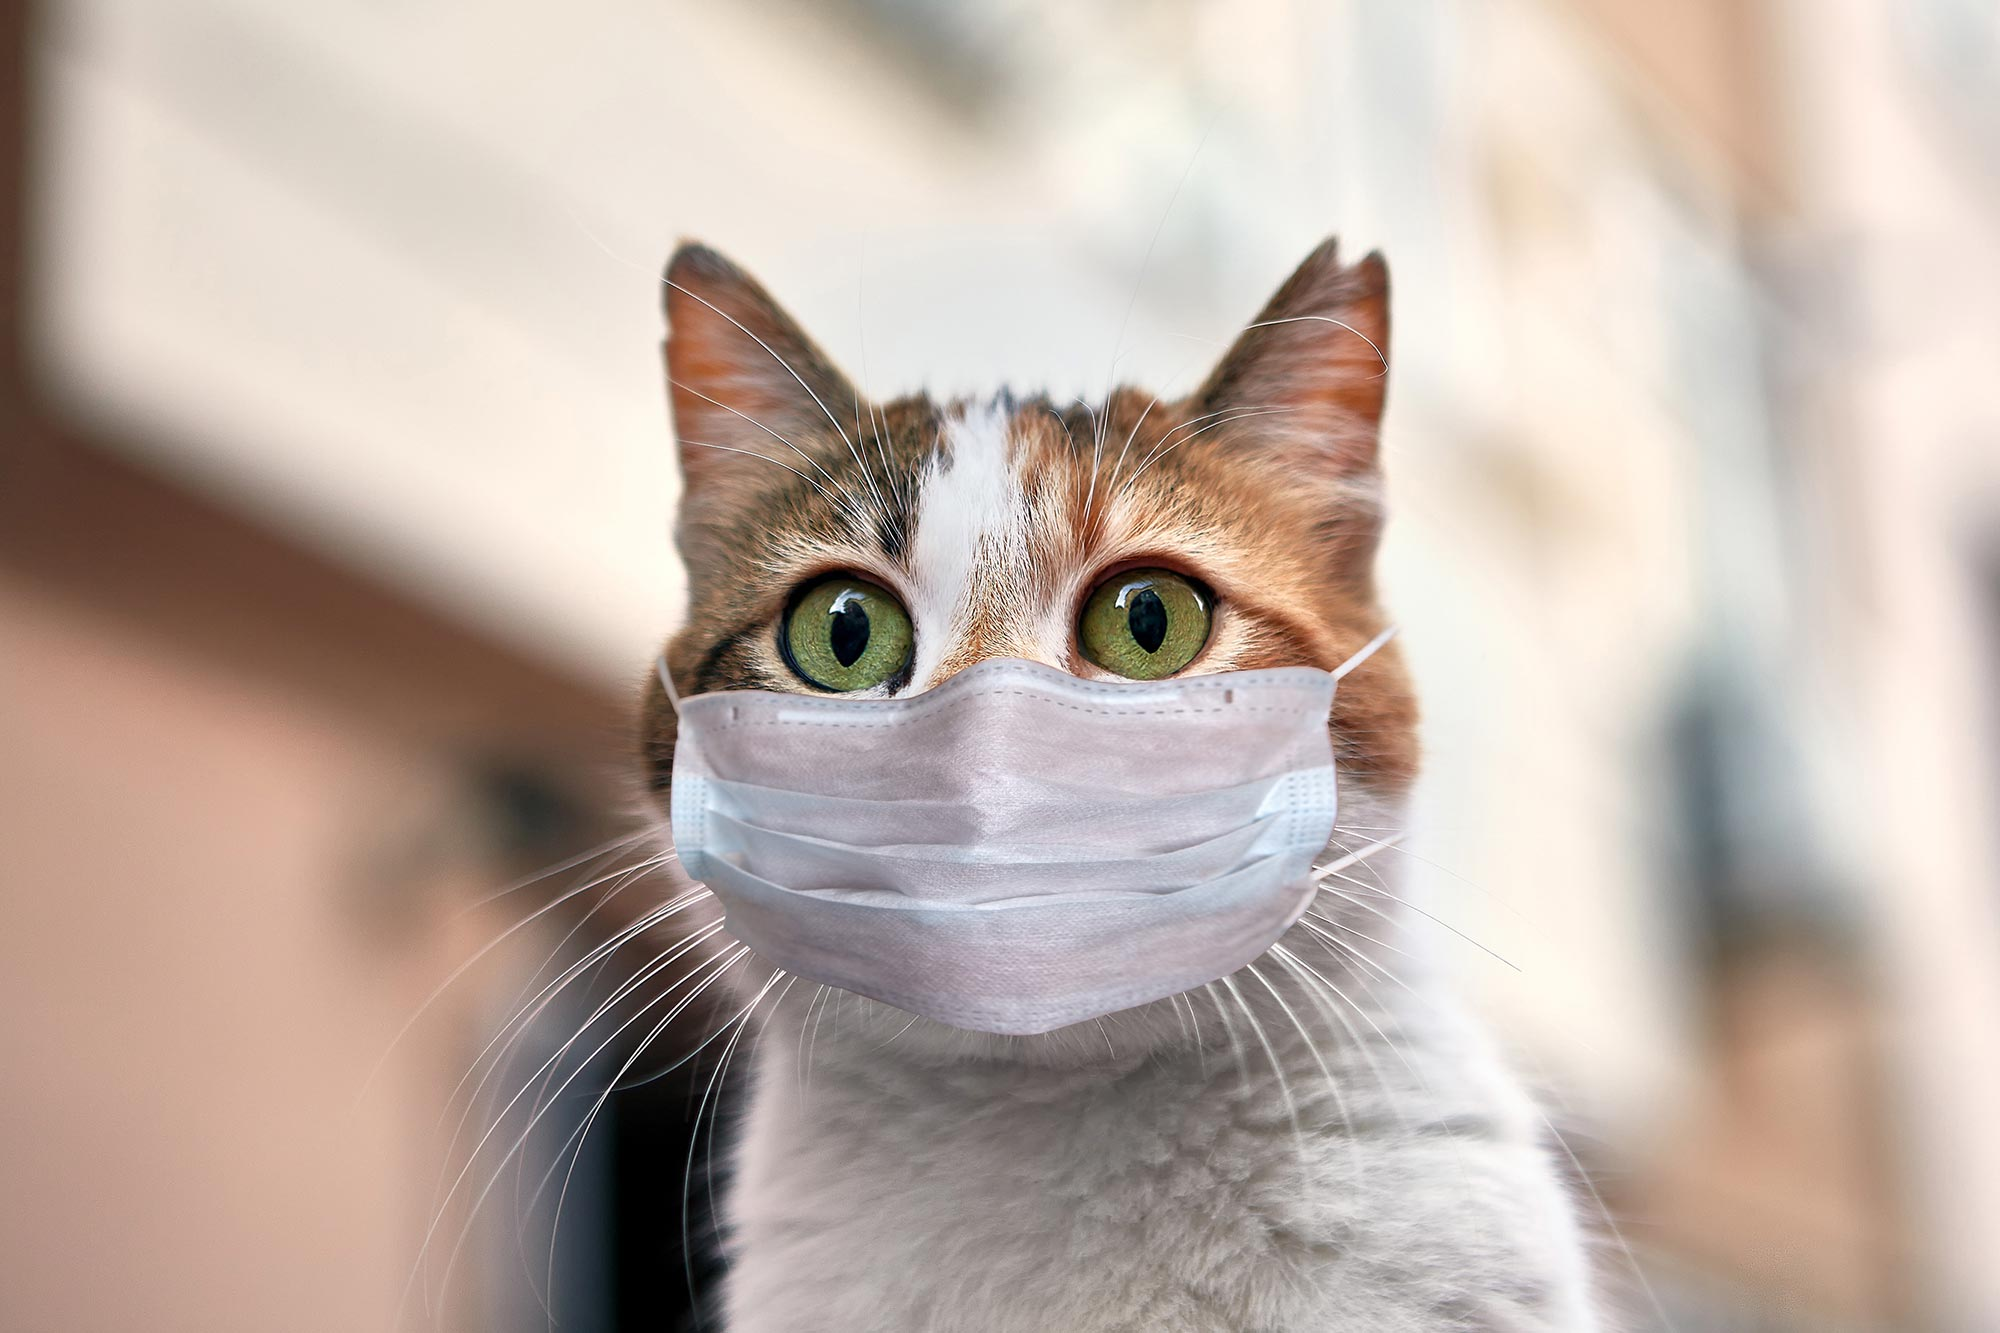
\includegraphics[width=0.5\linewidth]{images/cat.jpg}
        \caption{This is a description of the figure.}\label{fig:cat}
    \end{figure}
\end{outputbox}
\pagebreak
Providing a second dimension may skew the image:
\begin{minted}{tex}
\begin{figure}[H]
    \centering
    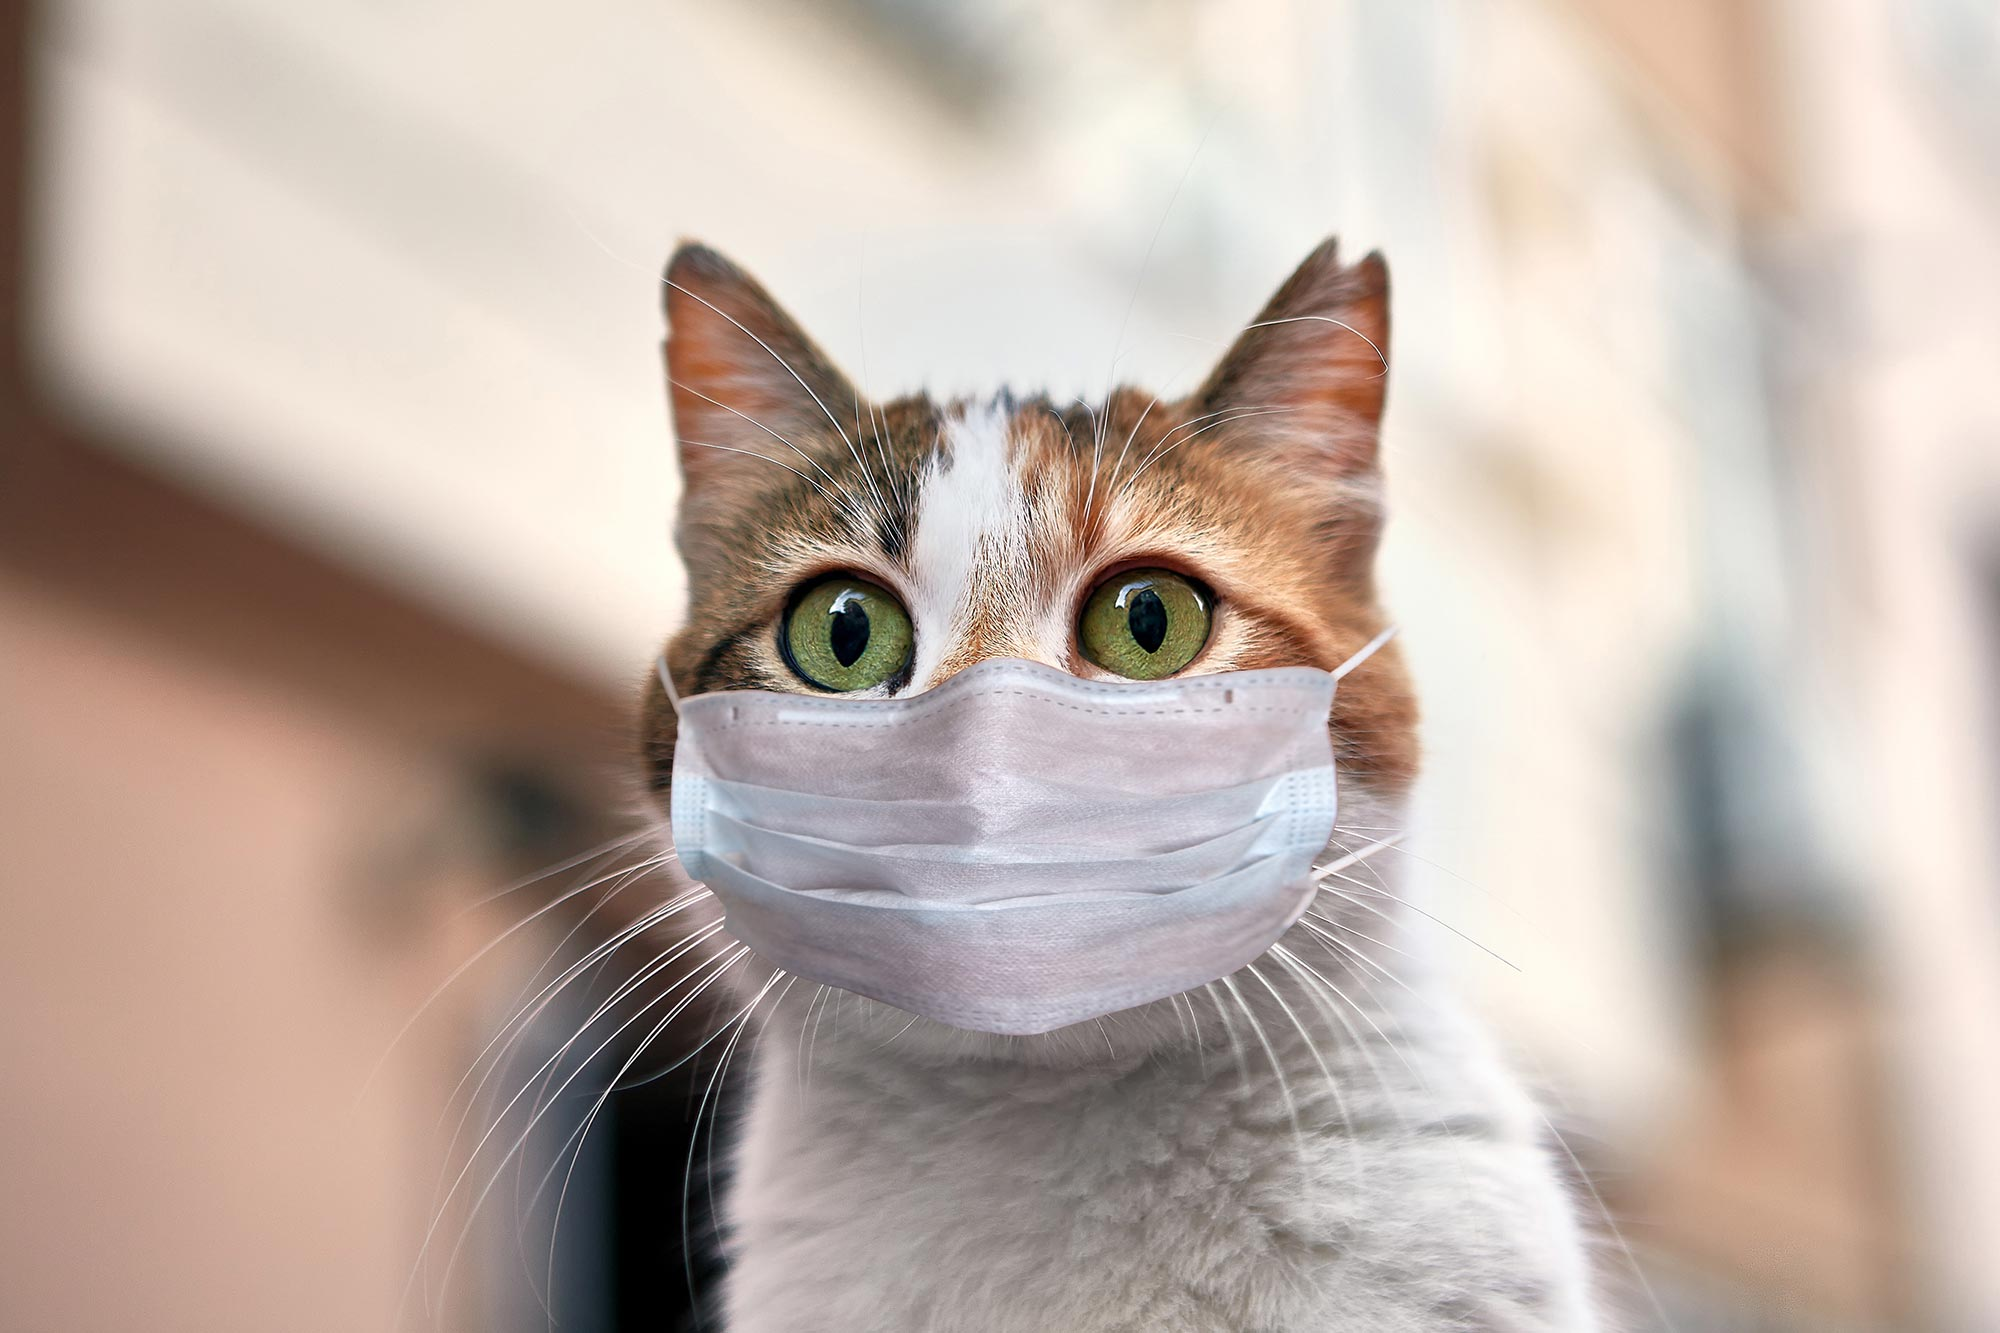
\includegraphics[width=1cm, height=5cm]{images/cat.jpg}
    \caption{Skewed image of cat.}
\end{figure}
\end{minted}
\begin{outputbox}
    \begin{figure}[H]
        \centering
        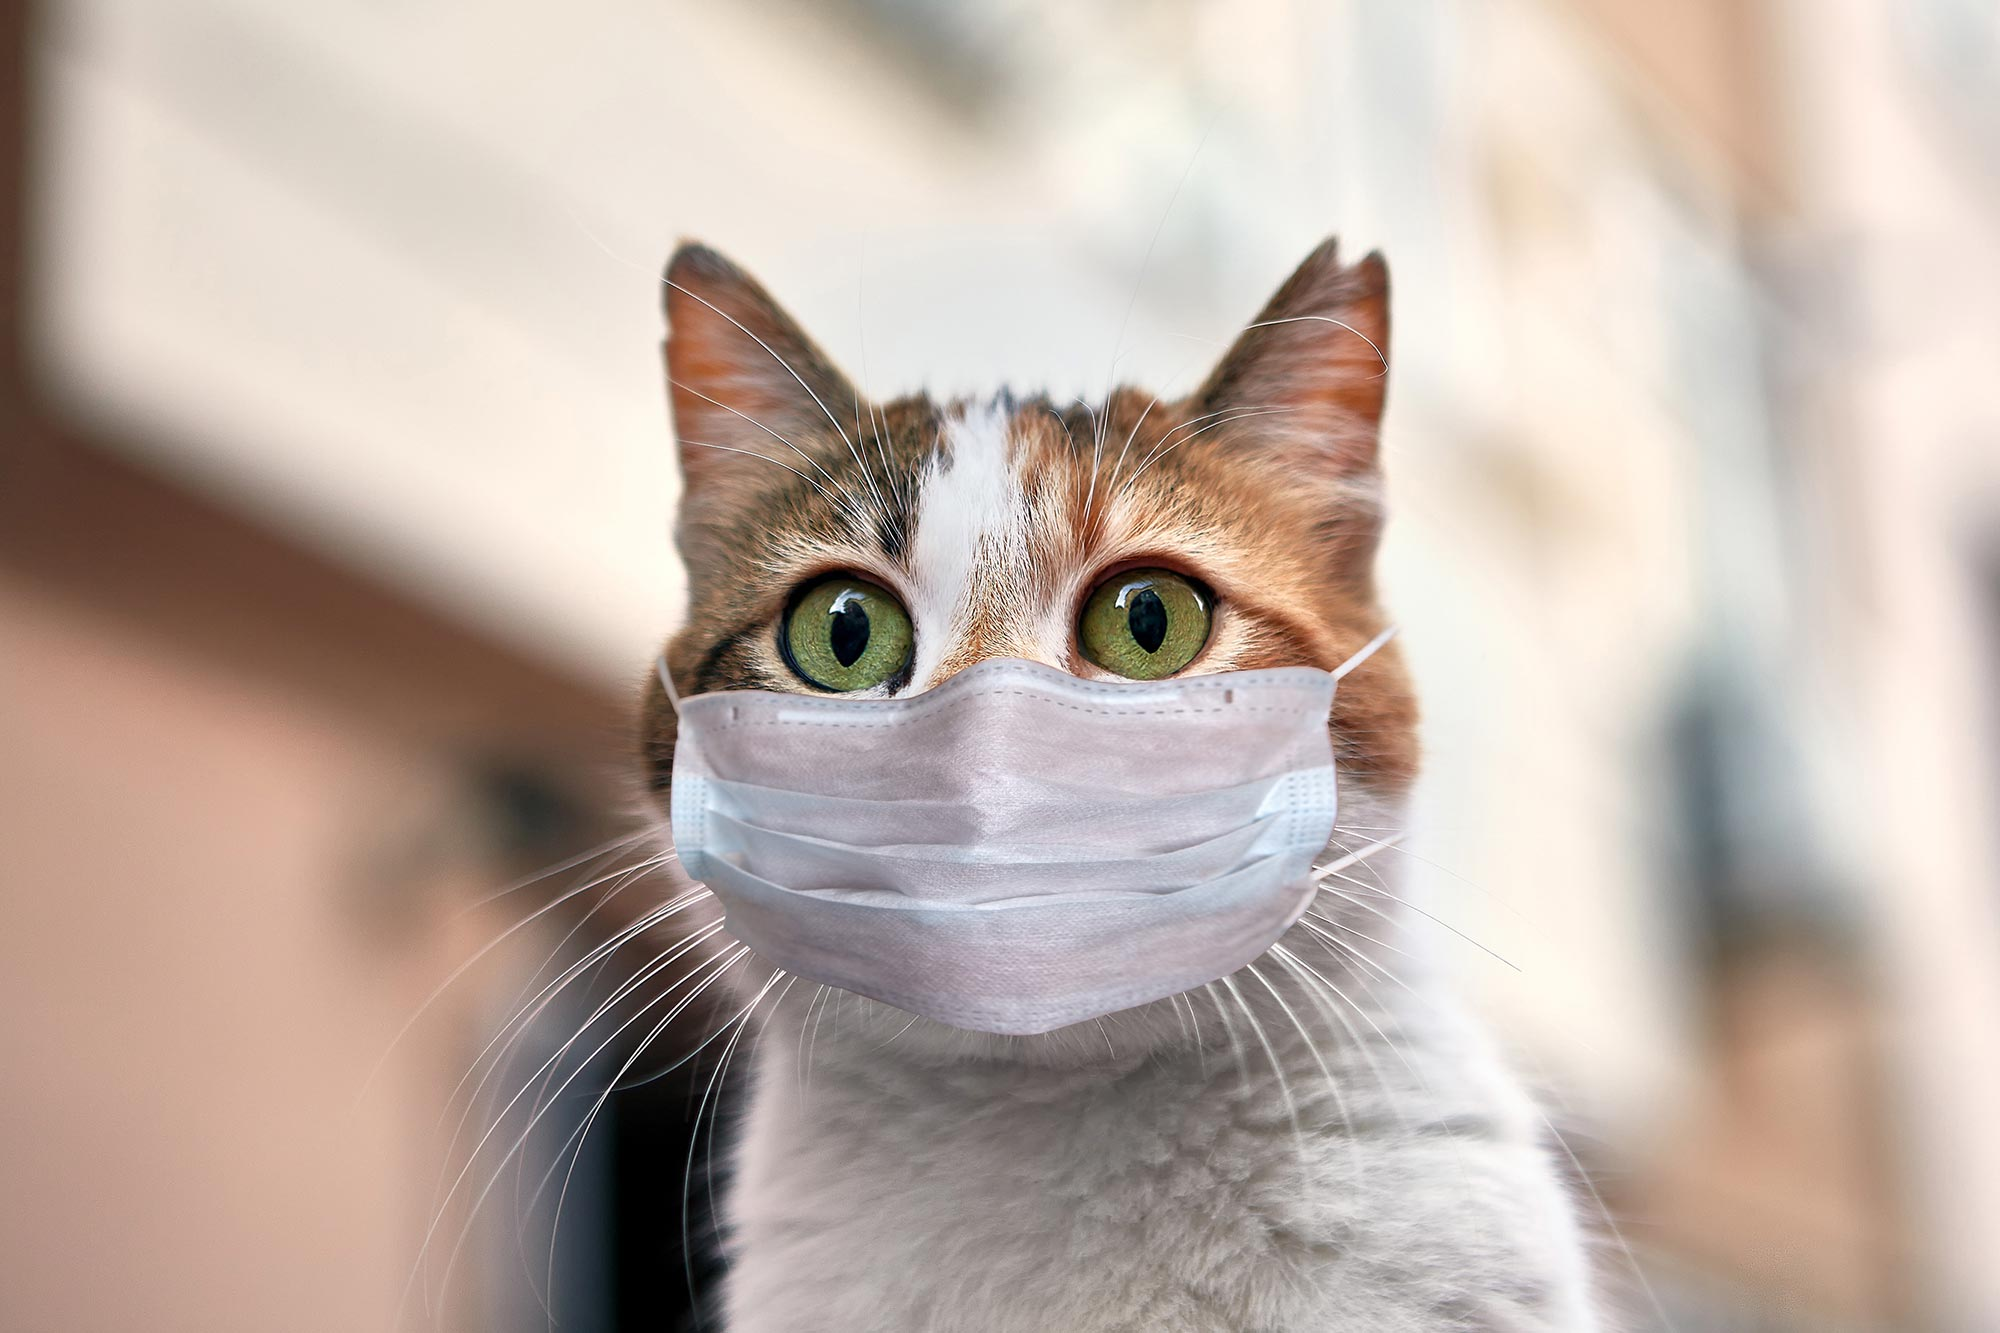
\includegraphics[width=1cm, height=5cm]{images/cat.jpg}
        \caption{Skewed image of cat.}
    \end{figure}
\end{outputbox}
An example using the \mintinline{tex}{subfigure} environment.
\begin{minted}{tex}
\begin{figure}[H]
    \centering
    \begin{subfigure}{0.47\linewidth}
        \centering
        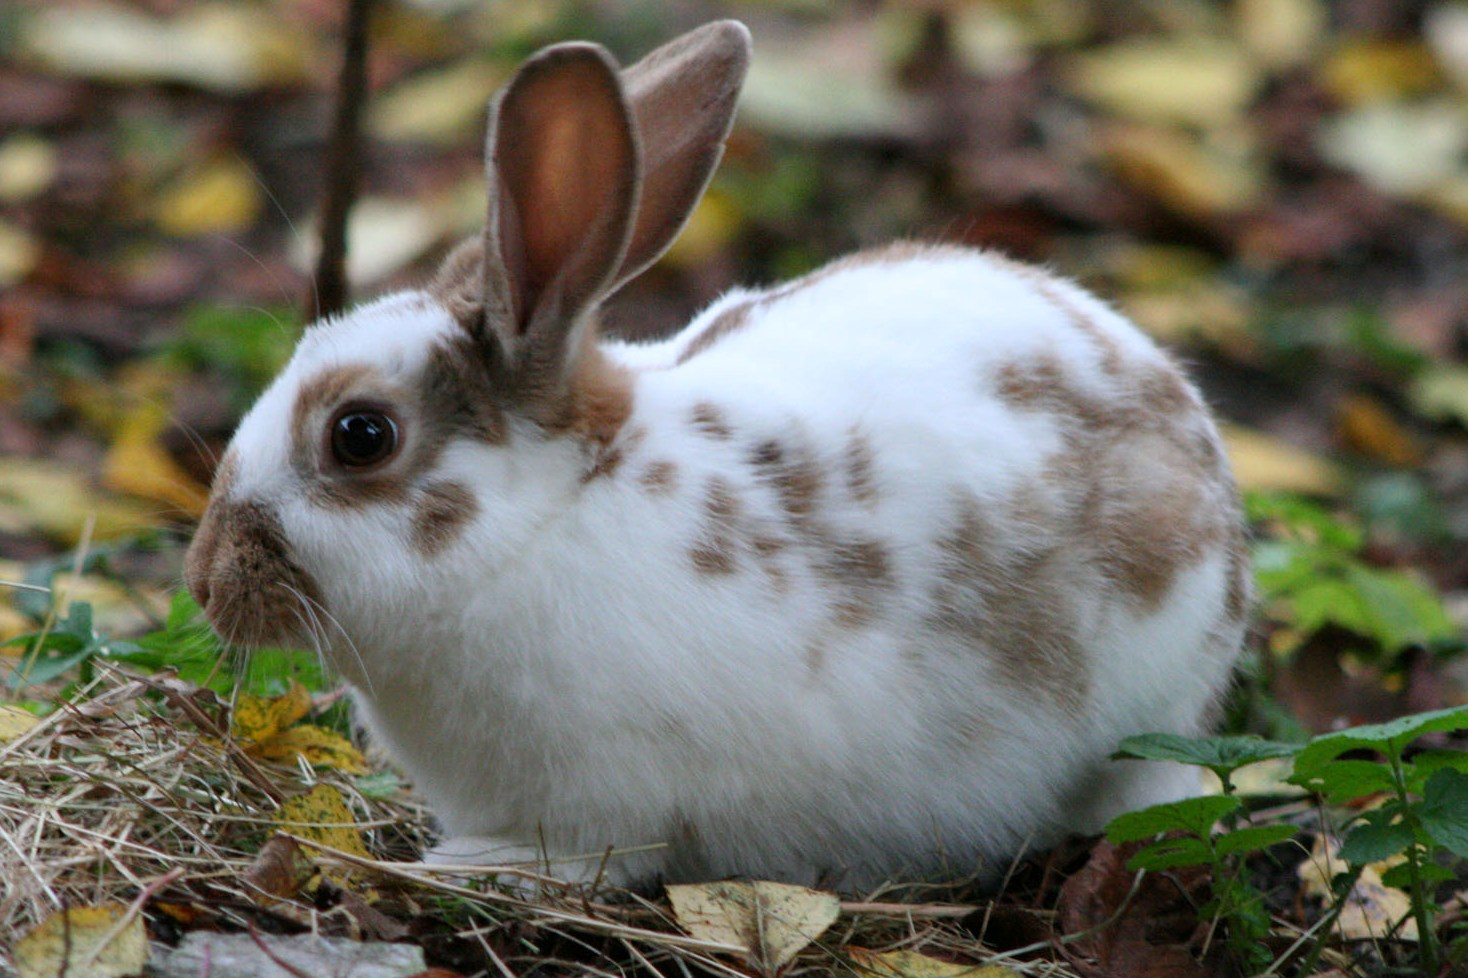
\includegraphics[height=3.5cm]{images/rabbit.jpg}
        \caption{The first subfigure.}
    \end{subfigure}
    \begin{subfigure}{0.47\linewidth}
        \centering
        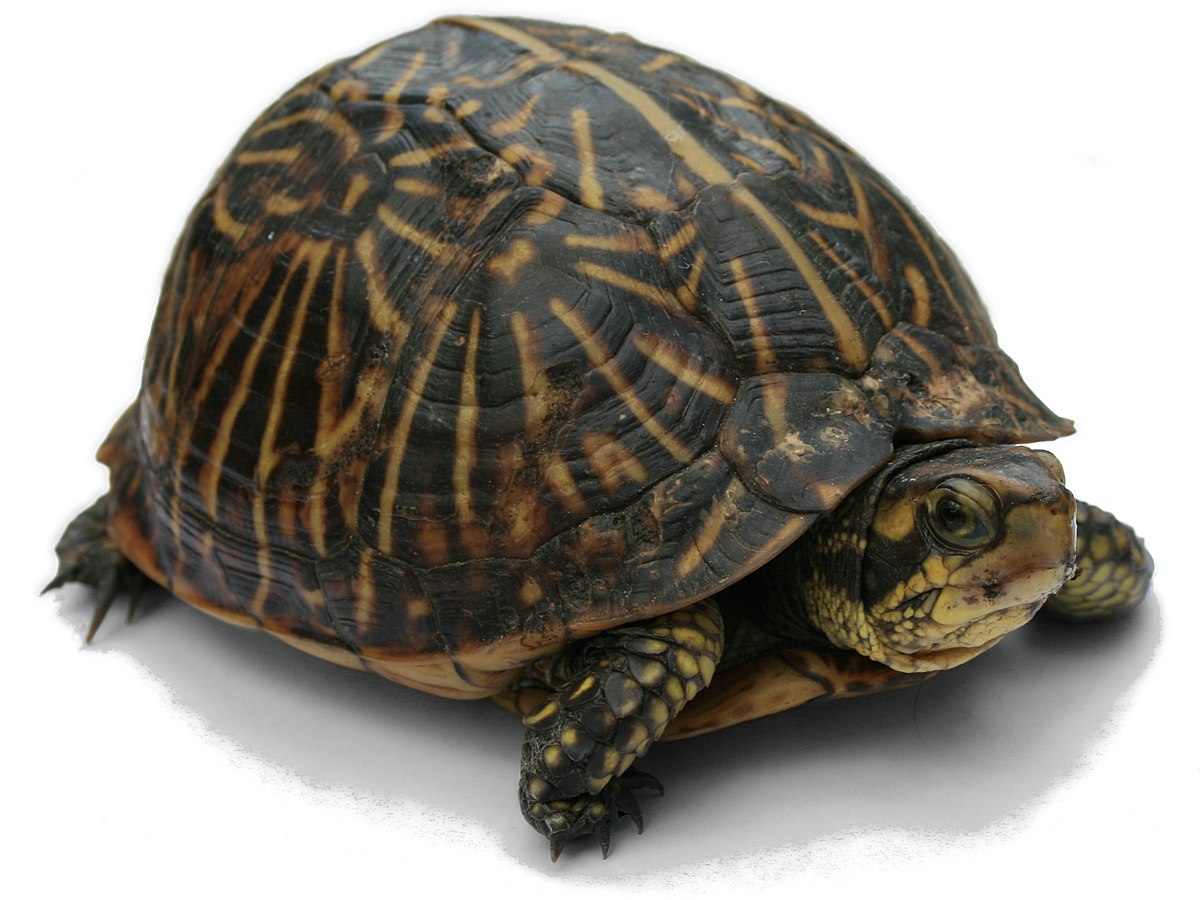
\includegraphics[height=3.5cm]{images/turtle.jpg}
        \caption{The second subfigure.}\label{fig:turtle}
    \end{subfigure}
    \caption{A description for both subfigures.}
\end{figure}
\end{minted}
\begin{outputbox}
    \begin{figure}[H]
        \centering
        \begin{subfigure}{0.47\linewidth}
            \centering
            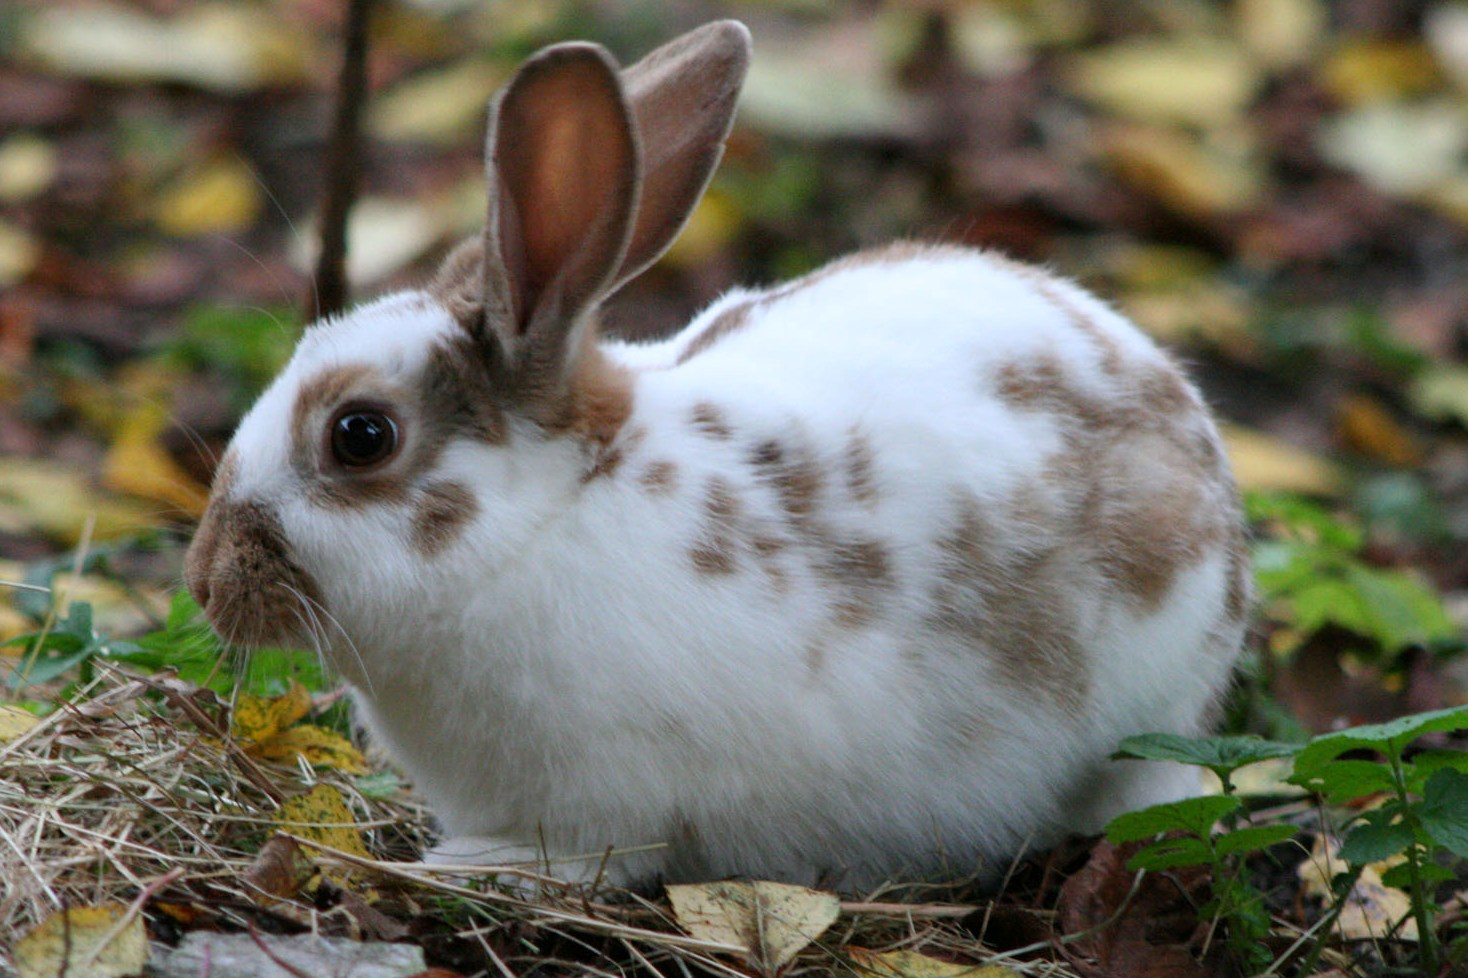
\includegraphics[height=3.5cm]{images/rabbit.jpg}
            \caption{The first subfigure.}
        \end{subfigure}
        \begin{subfigure}{0.47\linewidth}
            \centering
            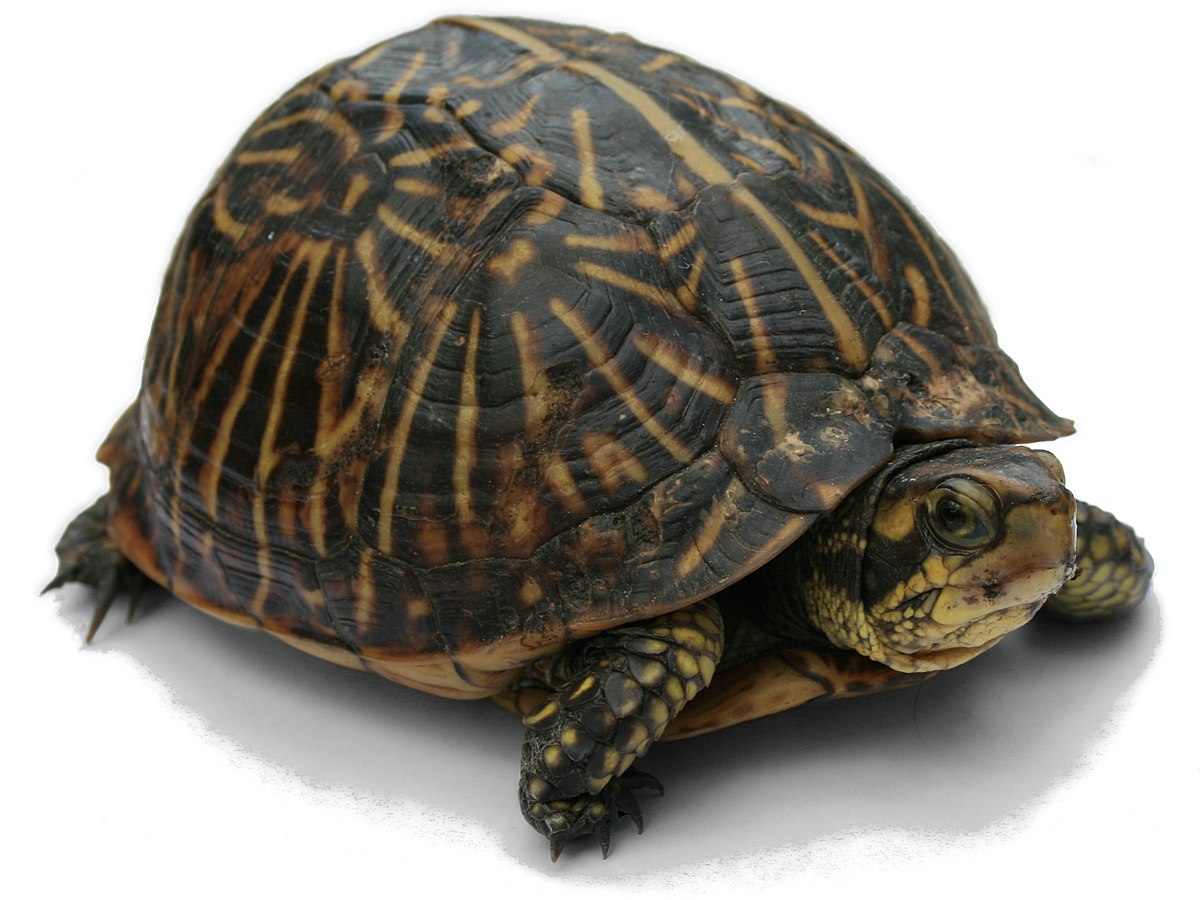
\includegraphics[height=3.5cm]{images/turtle.jpg}
            \caption{The second subfigure.}\label{fig:turtle}
        \end{subfigure}
        \caption{A caption for both subfigures.}
    \end{figure}
\end{outputbox}
\pagebreak
An example of a table:
\begin{minted}{tex}
\begin{table}[H]
    \centering
    \caption{Table descriptions precede the table.}\label{tab:table}
    \begin{tabular}{l c r}
        \toprule
        \textbf{Column 1} & \textbf{Column 2} & \textbf{Column 3} \\
        \midrule
        3                 & 1                 & 4                 \\
        1                 & 5                 & 9                 \\
        2                 & 6                 & 5                 \\
        3                 & 5                 & 8                 \\
        \bottomrule
    \end{tabular}
\end{table}
\end{minted}
\begin{table}[H]
    \centering
    \caption{Table descriptions precede the table.}\label{tab:table}
    \begin{tabular}{l c r}
        \toprule
        \textbf{Column 1} & \textbf{Column 2} & \textbf{Column 3} \\
        \midrule
        3                 & 1                 & 4                 \\
        1                 & 5                 & 9                 \\
        2                 & 6                 & 5                 \\
        3                 & 5                 & 8                 \\
        \bottomrule
    \end{tabular}
\end{table}
Note that we also use the \mintinline{tex}{\centering} macro to horizontally centre the contents of the floats.
\subsection{List of Figures and Tables}
A list of figures and tables can be printed with
\mintinline{tex}{\listoffigures} and \mintinline{tex}{\listoftables}.
These are similar to the table of contents.
\subsection{Code}
Source code can be displayed using the \mintinline{tex}{minted}
environment and in addition to the environment, code can also be
displayed inline with the \mintinline{tex}{\mintinline{tex}} macro
(this is how code has been formatted throughout this document).
\begin{minted}[escapeinside=||]{tex}
\begin{minted}{cpp}
#include <iostream>

int main() {
    std::cout << "Hello World!" << std::endl;
    return 0
}
\end||{minted}
\end{minted}
\begin{outputbox}
    \begin{minted}{cpp}
#include <iostream>

int main() {
    std::cout << "Hello World!" << std::endl;
    return 0;
}
\end{minted}
\end{outputbox}
Example inline code:
\begin{minted}{tex}
The \mintinline{tex}{System.Double} class is used for double precision floating-point values.
\end{minted}
\begin{outputbox}
    The \mintinline{tex}{System.Double} class is used for double precision floating-point values.
\end{outputbox}
If the inline code contains braces (\mintinline{tex}|{ }|), we need to delineate the argument using another symbol.
\begin{minted}{tex}
We define the array: \mintinline{tex}|int[] array = { 1, 2, 3 }|.
\end{minted}
\begin{outputbox}
    We define the array: \mintinline{tex}|int[] array = { 1, 2, 3 }|.
\end{outputbox}
Here we can use the same symbol to delineate the arguments inside the
macro. In this case we use pipes (\mintinline{tex}{|}), but we can use
any symbol apart from the percentage sign (\%), i.e., \linebreak
\mintinline{tex}|\mintinline{tex}%code%| will not compile.
\subsection{References \& Labels}
Throughout this document, many elements are numbered (e.g.\ equations,
sections, figures, tables, etc.).

These elements (and others) can be marked using the
\mintinline{tex}{\label} macro. This marker can then be referenced
anywhere in the document (even before it is defined) with the
\mintinline{tex}{\ref} macro, and its page number can be obtained
through the \mintinline{tex}{\pageref} macro.

The examples in Section~\ref{sec:figures_and_tables} contained many
caption markers, and the following example will show how they are
referenced.
\begin{minted}{tex}
\begin{itemize}
    \item Cat figure: Figure~\ref{fig:cat}
    \item Turtle subfigure: Figure~\ref{fig:turtle}
    \item Example table: Table~\ref{tab:table}
    \item Schrödinger's equation: Equation~\ref{eq:schrodingers_equation}
    \item Figures \& Tables subsection: Section~\ref{sec:figures_and_tables} on Page~\pageref{sec:figures_and_tables}
\end{itemize}
\end{minted}
\begin{outputbox}
    \begin{itemize}
        \item Cat figure: Figure~\ref{fig:cat}
        \item Turtle subfigure: Figure~\ref{fig:turtle}
        \item Example table: Table~\ref{tab:table}
        \item Schrödinger's equation:
              Equation~\ref{eq:schrodingers_equation}
        \item Figures \& Tables subsection:
              Section~\ref{sec:figures_and_tables} on
              Page~\pageref{sec:figures_and_tables}
    \end{itemize}
\end{outputbox}
If we were to add an additional label, \LaTeX{} will automatically renumber all existing references the next time we compile the document.
\subsubsection{Hyperlinks}
We recommend using the \mintinline{tex}{hyperref} package to convert
references into hyperlinks for easy navigation on a PDF viewer. This
package also allows us to add custom text for references such as:
\begin{minted}{tex}
See the \LaTeX{} Project \href{https://www.latex-project.org/}{here}.

View \hyperref[eq:schrodingers_equation]{Schrödinger's Equation}.
\end{minted}
\begin{outputbox}
    See the \LaTeX{} Project \href{https://www.latex-project.org/}{here}.

    View \hyperref[eq:schrodingers_equation]{Schrödinger's Equation}.
\end{outputbox}
\newpage
\section{Diagrams}
If we wish to generate simple plots of functions, or complex diagrams,
we can do so with \LaTeX{} itself. The \mintinline{tex}{tikz} library
provides a multitude of packages for various kinds of diagrams.
\begin{figure}[H]
    \centering
    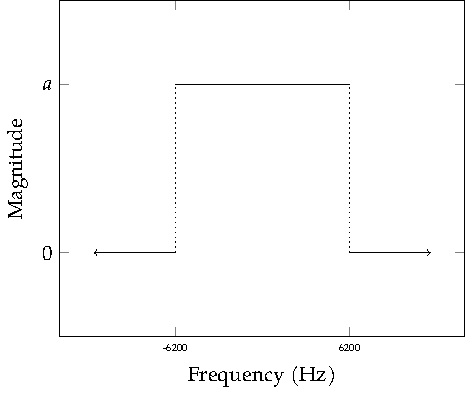
\includegraphics[height = 6.5cm]{figures/frequency_plot.pdf}
    \caption{Band pass filter.}
\end{figure}
\begin{figure}[H]
    \centering
    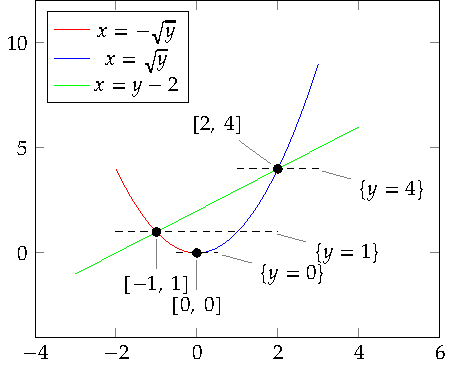
\includegraphics[height = 6.5cm]{figures/graph.pdf}
    \caption{Graph of three functions.}
\end{figure}
\begin{figure}[H]
    \centering
    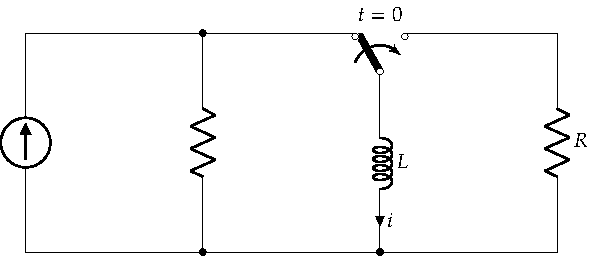
\includegraphics[width = 0.7\linewidth]{figures/circuit.pdf}
    \caption{RL circuit.}
\end{figure}
\newpage
\section{Citations, Bibliographies \& Reference Lists}
There are many ways to manage citations, bibliographies, and reference
lists in \LaTeX{}. This document will introduce a method that combines
BibLaTeX with Biber.

BibLaTeX is the frontend in \LaTeX{} that prints the bibliography and
Biber is the backend that manages the database which contains all
references.

When importing the \mintinline{tex}{biblatex} package we must supply
the reference style as follows:
\begin{minted}{tex}
\usepackage[style=APA]{biblatex}
\end{minted}
This affects both the citations and bibliography.

The references are stored in a Bibliographical Database file that uses
the \directory{.bib} extension. A sample database file has been
provided in the project directory.

The database file is added with
\begin{minted}{tex}
\addbibresource{path/to/database.bib}
\end{minted}
To cite the sources in this file, we can use the following macros:
\begin{minted}{tex}
\cite{reference_name}
\parencite{reference_name}
\end{minted}
For example:
\begin{minted}{tex}
Source 1 ---~\parencite{colu92}

Source 2 ---~\cite{phil99}
\end{minted}
\begin{outputbox}
    Source 1 ---~\parencite{colu92}

    Source 2 ---~\cite{phil99}
\end{outputbox}
The bibliography can be printed with the \mintinline{tex}{\printbibliography} macro, which will only print sources that are cited in the document.
\newpage
\section{Miscellaneous}
\subsection{Horizontal Spacing}
The following macros control horizontal spacing:
\begin{minted}{tex}
\begin{align*}
    A & \!     B \\
    A &        B \\
    A & \,     B \\
    A & \:     B \\
    A & \;     B \\
    A & \      B \\
    A & \quad  B \\
    A & \qquad B
\end{align*}
\end{minted}
\begin{outputbox}
    \begin{align*}
        A & \!     B \\
        A & B        \\
        A & \,     B \\
        A & \:     B \\
        A & \;     B \\
        A & \      B \\
        A & \quad  B \\
        A & \qquad B
    \end{align*}
\end{outputbox}
\subsection{Managing Large Documents}
If we want to organise large \LaTeX{} project files, we can split our
source code up into multiple files using the \mintinline{tex}{\input}
macro.% chktex 27

The following example requires the file: \directory{src/extras.tex}. If
we place the following code in the document (right after this text),
then we should see an additional section appear.
\begin{minted}{tex}
\subsection{Extra Section}
Congrats you found the extra section! Here's a bonus equation:
\begin{equation}\label{eq:bonus}
    \psi^{\left( m \right)} \left( z \right) = \odv*[order={m + 1}]{\ln{\left( \Gamma\left( z \right) \right)}}{z} = \left( -1 \right)^{m + 1} \int_0^\infty \frac{t^m e^{-zt}}{1 - e^{-t}} \odif{t}
\end{equation}

\end{minted}
\begin{outputbox}
    \subsection{Extra Section}
Congrats you found the extra section! Here's a bonus equation:
\begin{equation}\label{eq:bonus}
    \psi^{\left( m \right)} \left( z \right) = \odv*[order={m + 1}]{\ln{\left( \Gamma\left( z \right) \right)}}{z} = \left( -1 \right)^{m + 1} \int_0^\infty \frac{t^m e^{-zt}}{1 - e^{-t}} \odif{t}
\end{equation}

\end{outputbox}
We can even reference the markers that were defined in this file:
\begin{minted}{tex}
The polygamma function is summarised by Equation~\ref{eq:bonus}.
\end{minted}
\begin{outputbox}
    The polygamma function is summarised by Equation~\ref{eq:bonus}.
\end{outputbox}
\newpage
\section{Other Resources}
\begin{itemize}
    \item \href{https://en.wikibooks.org/wiki/LaTeX}{Wikibooks} --- Reference documentation and guides
    \item \href{https://www.overleaf.com/learn/latex/Tutorials}{Overleaf} --- Reference documentation and guides
    \item \href{https://tex.stackexchange.com/}{The \TeX{} Stack Exchange} --- Q\&A site for both \LaTeX{} and typesetting issues
    \item \href{https://ctan.org/}{The Comprehensive \TeX{} Archive Network (CTAN)} --- Package database
\end{itemize}
\newpage
\printbibliography
\end{document}
